%package list
\documentclass{article}
\usepackage[top=3cm, bottom=3cm, outer=3cm, inner=3cm]{geometry}
\usepackage{multicol}
\usepackage{graphicx}
\usepackage{url}
%\usepackage{cite}
\usepackage{hyperref}
\usepackage{array}
%\usepackage{multicol}
\newcolumntype{x}[1]{>{\centering\arraybackslash\hspace{0pt}}p{#1}}
\usepackage{natbib}
\usepackage{pdfpages}
\usepackage{multirow}
\usepackage[normalem]{ulem}
\useunder{\uline}{\ul}{}
\usepackage{svg}
\usepackage{xcolor}
\usepackage{listings}
\lstdefinestyle{ascii-tree}{
    literate={├}{|}1 {─}{--}1 {└}{+}1 
  }
\lstset{basicstyle=\ttfamily,
  showstringspaces=false,
  commentstyle=\color{red},
  keywordstyle=\color{blue}
}
%\usepackage{booktabs}
\usepackage{caption}
\usepackage{subcaption}
\usepackage{float}
\usepackage{array}

\newcolumntype{M}[1]{>{\centering\arraybackslash}m{#1}}
\newcolumntype{N}{@{}m{0pt}@{}}


%%%%%%%%%%%%%%%%%%%%%%%%%%%%%%%%%%%%%%%%%%%%%%%%%%%%%%%%%%%%%%%%%%%%%%%%%%%%
%%%%%%%%%%%%%%%%%%%%%%%%%%%%%%%%%%%%%%%%%%%%%%%%%%%%%%%%%%%%%%%%%%%%%%%%%%%%
\newcommand{\itemEmail}{vmamanian@unsa.edu.pe}
\newcommand{\itemStudent}{Victor Mamani Anahua}
\newcommand{\itemCourse}{Fundamentos de la Programación II}
\newcommand{\itemCourseCode}{20230489}
\newcommand{\itemSemester}{II}
\newcommand{\itemUniversity}{Universidad Nacional de San Agustín de Arequipa}
\newcommand{\itemFaculty}{Facultad de Ingeniería de Producción y Servicios}
\newcommand{\itemDepartment}{Departamento Académico de Ingeniería de Sistemas e Informática}
\newcommand{\itemSchool}{Escuela Profesional de Ingeniería de Sistemas}
\newcommand{\itemAcademic}{2023 - B}
\newcommand{\itemInput}{Del 17 Octubre 2023}
\newcommand{\itemOutput}{Al 24 Octubre 2023}
\newcommand{\itemPracticeNumber}{07}
\newcommand{\itemTheme}{Laboratorio 07}
%%%%%%%%%%%%%%%%%%%%%%%%%%%%%%%%%%%%%%%%%%%%%%%%%%%%%%%%%%%%%%%%%%%%%%%%%%%%
%%%%%%%%%%%%%%%%%%%%%%%%%%%%%%%%%%%%%%%%%%%%%%%%%%%%%%%%%%%%%%%%%%%%%%%%%%%%

\usepackage[english,spanish]{babel}
\usepackage[utf8]{inputenc}
\AtBeginDocument{\selectlanguage{spanish}}
\renewcommand{\figurename}{Figura}
\renewcommand{\refname}{Referencias}
\renewcommand{\tablename}{Tabla} %esto no funciona cuando se usa babel
\AtBeginDocument{%
	\renewcommand\tablename{Tabla}
}

\usepackage{fancyhdr}
\pagestyle{fancy}
\fancyhf{}
\setlength{\headheight}{30pt}
\renewcommand{\headrulewidth}{1pt}
\renewcommand{\footrulewidth}{1pt}
\fancyhead[L]{\raisebox{-0.2\height}{
\includegraphics[width=3cm]{img/logo_episunsa.png}}}
\fancyhead[C]{\fontsize{7}{7}\selectfont	\itemUniversity \\ \itemFaculty \\ \itemDepartment \\ \itemSchool \\ \textbf{\itemCourse}}
\fancyhead[R]{\raisebox{-0.2\height}{
\includegraphics[width=1.2cm]{img/logo_abet}}}
\fancyfoot[L]{Estudiante Victor Mamani A.}
\fancyfoot[C]{\itemCourse}
\fancyfoot[R]{Página \thepage}

% para el codigo fuente
\usepackage{listings}
\usepackage{color, colortbl}
\definecolor{dkgreen}{rgb}{0,0.6,0}
\definecolor{gray}{rgb}{0.5,0.5,0.5}
\definecolor{mauve}{rgb}{0.58,0,0.82}
\definecolor{codebackground}{rgb}{0.95, 0.95, 0.92}
\definecolor{tablebackground}{rgb}{0.8, 0, 0}

\lstdefinestyle{java}{frame=tb,
	language=Java,
	showstringspaces=false,
	columns=flexible,
	basicstyle={\footnotesize\ttfamily\color[RGB]{255,255,255}},
	numberstyle=\color{mygray},
	numbers=left, 
	keywordstyle=\color{myblue},
	morekeywords={String, System},
	commentstyle=\color{mygray},
	stringstyle=\color{mygreen},
	breaklines=true,
	breakatwhitespace=true,
	tabsize=2,
	backgroundcolor= \color{codebackgroundCode},
	showspaces=false,
	showtabs=false,
	showlines=false,
}

\lstset{frame=tb,
	language=bash,
	aboveskip=3mm,
	belowskip=3mm,
	showstringspaces=false,
	columns=flexible,
	basicstyle={\small\ttfamily},
	numbers=none,
	numberstyle=\tiny\color{gray},
	keywordstyle=\color{blue},
	commentstyle=\color{dkgreen},
	stringstyle=\color{mauve},
	breaklines=true,
	breakatwhitespace=true,
	tabsize=3,
	backgroundcolor= \color{codebackground},
}

\begin{document}
	
	\vspace*{10px}
	
	\begin{center}	
		\fontsize{17}{17} \textbf{ Informe de Laboratorio \itemPracticeNumber}
	\end{center}
	\centerline{\textbf{\Large Tema: \itemTheme}}
	%\vspace*{0.5cm}	

	\begin{flushright}
		\begin{tabular}{|M{2.5cm}|N|}
			\hline 
			\rowcolor{tablebackground}
			\color{white} \textbf{Nota}  \\
			\hline 
			     \\[30pt]
			\hline 			
		\end{tabular}
	\end{flushright}	

	\begin{table}[H]
		\begin{tabular}{|x{4.7cm}|x{4.8cm}|x{4.8cm}|}
			\hline 
			\rowcolor{tablebackground}
			\color{white} \textbf{Estudiante} & \color{white}\textbf{Escuela}  & \color{white}\textbf{Asignatura}   \\
			\hline 
			{\itemStudent \par \itemEmail} & \itemSchool & {\itemCourse \par Semestre: \itemSemester \par Código: \itemCourseCode}     \\
			\hline 			
		\end{tabular}
	\end{table}		
	
	\begin{table}[H]
		\begin{tabular}{|x{4.7cm}|x{4.8cm}|x{4.8cm}|}
			\hline 
			\rowcolor{tablebackground}
			\color{white}\textbf{Laboratorio} & \color{white}\textbf{Tema}  & \color{white}\textbf{Duración}   \\
			\hline 
			\itemPracticeNumber & \itemTheme & 04 horas   \\
			\hline 
		\end{tabular}
	\end{table}
	
	\begin{table}[H]
		\begin{tabular}{|x{4.7cm}|x{4.8cm}|x{4.8cm}|}
			\hline 
			\rowcolor{tablebackground}
			\color{white}\textbf{Semestre académico} & \color{white}\textbf{Fecha de inicio}  & \color{white}\textbf{Fecha de entrega}   \\
			\hline 
			\itemAcademic & \itemInput &  \itemOutput  \\
			\hline 
		\end{tabular}
	\end{table}
	
	\section{Tarea}
	\begin{itemize}		
        \item Cree un Proyecto llamado Laboratorio7
		\item Usted deberá crear las dos clases Soldado.java y VideoJuego4.java. Puede reutilizar lo desarrollado en Laboratorios anteriores.
		\item Del Soldado nos importa el nombre, puntos de vida, fila y columna (posición en el tablero).
		\item El juego se desarrollará en el mismo tablero de los laboratorios anteriores. Para el tablero utilizar la estructura de datos más adecuada.
		\item Tendrá 2 Ejércitos. Inicializar el tablero con n soldados aleatorios entre 1 y 10 para cada Ejército. Cada soldado tendrá un nombre autogenerado: Soldado0X1, Soldado1X1, etc., un valor de puntos de vida autogenerado aleatoriamente [1..5], la fila y columna también autogenerados aleatoriamente (no puede haber 2 soldados en el mismo cuadrado). 
		\item Además de los datos del Soldado con mayor vida de cada ejército, el promedio de puntos de vida de todos los soldados creados por ejército, los datos de todos los soldados porejército en el orden que fueron creados y un ranking de poder de todos los soldados creados por ejército (del que tiene más nivel de vida al que tiene menos) usando 2 diferentes algoritmos de ordenamiento.
		\item Finalmente, que muestre qué ejército ganará la batalla (indicar la métrica usada para decidir al ganador de la batalla).
	\end{itemize}

	\section{Equipos, materiales y temas utilizados}
	\begin{itemize}
		\item Sistema Operativo Ubuntu GNU Linux 23 lunar 64 bits Kernell 6.2.v
		\item Visual Studio Code.
		\item VIM 9.0.
		\item OpenJDK 64-Bits 19.0.7.
		\item Git 2.39.2.
		\item Cuenta en GitHub con el correo institucional.
		\item Programación Orientada a Objetos.
		\item Actividades del Laboratorio 07.	
	\end{itemize}
	
	\section{URL de Repositorio Github}
	\begin{itemize}
		\item URL del Repositorio GitHub para clonar o recuperar.
		\item \url{https://github.com/VictorMA18/fp2-23b.git}
		\item URL para el laboratorio 07 en el Repositorio GitHub.
		\item \url{https://github.com/VictorMA18/fp2-23b/tree/main/Fase02/Lab07}
	\end{itemize}
	
	\section{Actividades del Laboratorio 07}
	
	\subsection{Ejercicio Soldado}
	\begin{itemize}	
		\item En el primer commit bueno reutilizamos el archivo que seria nuestra clase Soldado el cual la utilizaremos para poder avanzar con el siguiente ejercicio que seria VideoJuego4.
		\item El codigo y el commit seria el siguiente:
	\end{itemize}	
	\begin{lstlisting}[language=bash,caption={Commit}][H]
		$ git commit -m "Publicando la clase soldado para el ejercicio7 la cual es la clase soldado donde estan los atributos mas importantes que nos serviran"
	\end{lstlisting}	
	\begin{lstlisting}[language=java,caption={Las lineas de codigos del metodo creado:}][H]
		// Laboratorio Nro 7  - Ejercicio Soldado
		// Autor: Mamani Anahua Victor Narciso
		// Colaboro:
		// Tiempo:
		public class Soldado { //CREAMOS LA CLASE SOLDODADO PARA PODER USAR UN ARREGLO BIDIMENSIONAL DONDE NECESITAMOS LA VIDA , EL NOMBRE DEL SOLDADO Y TAMBIEN SU POSICION COMO LA FILA Y LA COLUMNA   

			private String name;
			private int heatlh; 
			private int row;
			private String column;

			//Constructor
			public Soldado(String name, int health, int row, String column){
			this.name = name;
			this.health = health;
			this.row = row;
			this.column = column;
			}

			// Metodos mutadores
			public void setName(String n){
				name = n;
			}
			public void setHealth(int p){
				heatlh = p;
			}
			public void setRow(int b){
				row = b;
			}
			public void setColumn(String c){
				column = c; 
			}

			// Metodos accesores
			public String getName(){
				return name;
			}
			public int getHealth(){
				return heatlh;

			}
			public int getRow(){
				return row;
			}
			public String getColumn(){
				return column;
			}

			// Completar con otros metodos necesarios
			public String toString(){ //CREAMOS ESTE METODO PARA IMPRIMIR LOS DATOS DEl OBJETO
				String join = "\nNombre: " + getName() + "\nVida: " + getHealth() + "\nFila: " + getRow() + "\nColumna: " + getColumn(); //Agregamos un espaciador para poder separar
				return join;
			}
		}
	\end{lstlisting}
	\subsection{Ejercicio VideoJuego4}
	\begin{itemize}	
		\item En el segundo commit completamos el metodo arrayfillregister() el cual queremos rellenar el array de soldados del ejercito 2 para poder verlos en el tablero a la ves su informacion de cada soldado el cual va hacer por orden de creacion
		\item El codigo , el commit y la ejecucion seria el siguiente:
	\end{itemize}	
	\begin{lstlisting}[language=bash,caption={Commit}][H]
		$ git commit -m "Creando el metodo arrayfillregister() para que este pueda imprimir los datos de los soldados que estan en el tablero este te devuelve el array lleno con la cantidad de soldados y texto que dice su informacion de cada soldado Y tambien cumplimos con el cual no se repita un soldado en el mismo casillero ya que al ver que este lleno este retrocedera una repeticion ya que estaria tomando la repeticion en un casillero lleno"
	\end{lstlisting}	
	\begin{lstlisting}[language=java,caption={Las lineas de codigos del metodo creado:}][H]
		public static Soldado[][] arrayfillregister(int num){ //METODO CREADO PARA PODER CREAR AL EJERCITO 2 EL CUAL USAREMOS LA ESTRUCTURA DE DATO QUE ES EL ARRAY CON TAL QUE TAMBIEN REGISTRAMOS 
			Random rdm = new Random();
			int numsoldiers = rdm.nextInt(10) + 1;
			System.out.println("La Ejercito " + num + " tiene " + numsoldiers + " soldados:");  
			System.out.println("*********************************");
			Soldado[][] army = new Soldado[10][10];
			for(int i = 0; i < numsoldiers; i++){ //LOS REGISTRAMOS A CADA UNO POR EL ORDEN DE CREACION QUE FUERON CREADOS EL CUAL TAMBIEN COMPLETAMOS SUS DATOS Y LOS PUBLICAMOS POR ORDEN 
				System.out.println("Registrando al " + (i + 1) + " soldado del Ejercito " + num + "");            
				String name = "Soldado" + i + "X" + num;            
				int health = rdm.nextInt(5) + 1;
				int row = rdm.nextInt(10) + 1;
				String column = String.valueOf((char)(rdm.nextInt(10) + 65));  
				if(army[row - 1][(int)column.charAt(0) - 65] == null){ //VERIFICAMOS QUE NO SE REPITAN MISMOS SOLDADOS DE UN EJERCITO EN EL MISMO CUADRADO 
					System.out.print("------------------");
					army[row - 1][(int)column.charAt(0) - 65] = new Soldado(name, health, row, column);
					System.out.println(army[row - 1][(int)column.charAt(0) - 65].toString());
				}else{
					i -= 1;
				}
			}
			return army;
    	}
	\end{lstlisting}
	\begin{lstlisting}[language=bash,caption={Ejecucion:}][H]
		La Ejercito 2 tiene 6 soldados:
		*********************************
		Registrando al 1 soldado del Ejercito 2
		------------------
		Nombre: Soldado0X2
		Vida: 5
		Fila: 8
		Columna: C
		Registrando al 2 soldado del Ejercito 2
		------------------
		Nombre: Soldado1X2
		Vida: 5
		Fila: 2
		Columna: I
		Registrando al 3 soldado del Ejercito 2
		------------------
		Nombre: Soldado2X2
		Vida: 5
		Fila: 5
		Columna: F
		Registrando al 4 soldado del Ejercito 2
		------------------
		Nombre: Soldado3X2
		Vida: 5
		Fila: 2
		Columna: G
		Registrando al 5 soldado del Ejercito 2
		------------------
		Nombre: Soldado4X2
		Vida: 2
		Fila: 10
		Columna: G
		Registrando al 6 soldado del Ejercito 2
		------------------
		Nombre: Soldado5X2
		Vida: 4
		Fila: 9
		Columna: F
	\end{lstlisting}
	\subsection{Ejercicio VideoJuego4}
	\begin{itemize}	
		\item En el tercer commit creamos el metodo arrayListFillRegister() para que este pueda llenar los ArrayList que creamos para el ejercito 1 en este se creara un arraylist con casillas de soldados con datos nulos el cual se va ir llenando aleatoriamente con soldados y a la vez de esto nos mostrara por orden de creacion la informacion de los soldados a la vez tambien permitiriamos que cada casilla no se repita un mismo soldado ya que este sera verificado mediante si este casilla sea diferente a un soldado nulo
		\item El codigo , el commit y la ejecucion seria el siguiente:
	\end{itemize}	
	\begin{lstlisting}[language=bash,caption={Commit}][H]
		$ git commit -m "Creamos el metodo arrayListFillRegister() para que este pueda llenar los ArrayList que creamos para el ejercito 1 en este se creara un arraylist con casillas de soldados con datos nulos el cual se va ir llenando aleatoriamente con soldados y a la vez de esto nos mostrara por orden de creacion la informacion de los soldados a la vez tambien permitiriamos que cada casilla no se repita un mismo soldado ya que este sera verificado mediante si este casilla sea diferente a un soldado nulo"
	\end{lstlisting}	
	\begin{lstlisting}[language=java,caption={Las lineas de codigos del metodo creado:}][H]
		public  static ArrayList<ArrayList<Soldado>> arrayListFillRegister(int num){
			Random rdm = new Random();
			ArrayList<ArrayList<Soldado>> army = new ArrayList<ArrayList<Soldado>>();
			int numbersoldiers = rdm.nextInt(10) + 1;
			for(int i = 0; i < 10; i++){
				army.add(new ArrayList<Soldado>()); //LLENAMOS NUESTROS ARRAYLIST BIDIMENSIONAL CON CADA FILA PARA QUE CUMPLAN CON ESTRUCTURA DEL TABLERO
				for(int j = 0; j < 10 ; j++){
					army.get(i).add(null); // LLENAMOS CADA FILA DEL ARRAYLIST CON UN OBJETO SOLDADO CON TAL QUE ESTE SEA NULL PARA QUE SEPA QUE ESTE TIENE UNA CASILLA PERO NO HAY NADIE TODAVIA SE PUEDE LLENAR 
				}
			}
			System.out.println("El Ejercito " + num + " tiene " + numbersoldiers + " soldados : " ); 
			System.out.println("*********************************");
			for(int i = 0; i < numbersoldiers; i++){ //LLENAMOS CASILLAS CON CADA SOLDADO CREADO ALEATORIAMENTE
				String name = "Soldado" + i + "X" + num;
				int health = rdm.nextInt(5) + 1;
				int row = rdm.nextInt(10) + 1;
				String column = String.valueOf((char)(rdm.nextInt(10) + 65)); //REUTILIZAMOS CODIGO DEL ANTERIOR ARCHIVO VIDEOJUEGO3.JAVA YA QUE TENDRIAN LA MISMA FUNCIONALIDAD
				if(army.get(row - 1).get((int)column.charAt(0) - 65) == null){
					System.out.println("Registrando al " + (i + 1) + " soldado del Ejercito " + num + "");
					System.out.print("------------------");
					army.get(row - 1).set((int)column.charAt(0) - 65, new Soldado(name, health, row, column));
					System.out.println(army.get(row - 1).get((int)column.charAt(0) - 65).toString());
				}else{
					i -= 1; //NOS AYUDARIA CON LOS SOLDADOS QUE SE REPITEN EN EL MISMO CASILLERO CON TAL QUE NO DEBERIA CONTAR 
				}
			}
			System.out.println("*********************************");
			return army;
		}
	\end{lstlisting}
	\begin{lstlisting}[language=bash,caption={Ejecucion:}][H]
		El Ejercito 1 tiene 2 soldados : 
		*********************************
		Registrando al 1 soldado del Ejercito 1
		------------------
		Nombre: Soldado0X1
		Vida: 4
		Fila: 2
		Columna: F
		Registrando al 2 soldado del Ejercito 1
		------------------
		Nombre: Soldado1X1
		Vida: 2
		Fila: 8
		Columna: I
		*********************************

		El Ejercito 2 tiene 4 soldados:
		*********************************
		Registrando al 1 soldado del Ejercito 2
		------------------
		Nombre: Soldado0X2
		Vida: 1
		Fila: 4
		Columna: D
		Registrando al 2 soldado del Ejercito 2
		------------------
		Nombre: Soldado1X2
		Vida: 4
		Fila: 4
		Columna: H
		Registrando al 3 soldado del Ejercito 2
		------------------
		Nombre: Soldado2X2
		Vida: 2
		Fila: 7
		Columna: F
		Registrando al 4 soldado del Ejercito 2
		------------------
		Nombre: Soldado3X2
		Vida: 2
		Fila: 8
		Columna: I
	\end{lstlisting}
	\subsection{Ejercicio VideoJuego4}
	\begin{itemize}	
		\item En el cuarto commit creamos el metodo viewBoard() el cual nos dejaria permitir visualizar la tabla junto a su leyenda , con los soldados de cada ejercito su posicion la cual del ejercito 1 seria una x y el ejercito 2 seria una y en este tambien aplicamos para cada casilla la cual no sea nula poner una x para el ejercito 1 y en caso contrario debria ser del ejercito 2 el cual seria una y y si tambien seria en caso contrario seria nulo
		\item El codigo , el commit y la ejecucion seria el siguiente:
	\end{itemize}	
	\begin{lstlisting}[language=bash,caption={Commit}][H]
		$ git commit -m "Creamos el metodo arrayListFillRegister() para que este pueda llenar los ArrayList que creamos para el ejercito 1 en este se creara un arraylist con casillas de soldados con datos nulos el cual se va ir llenando aleatoriamente con soldados y a la vez de esto nos mostrara por orden de creacion la informacion de los soldados a la vez tambien permitiriamos que cada casilla no se repita un mismo soldado ya que este sera verificado mediante si este casilla sea diferente a un soldado nulo"
	\end{lstlisting}	
	\begin{lstlisting}[language=java,caption={Las lineas de codigos del metodo creado:}][H]
		public  static ArrayList<ArrayList<Soldado>> arrayListFillRegister(int num){
			Random rdm = new Random();
			ArrayList<ArrayList<Soldado>> army = new ArrayList<ArrayList<Soldado>>();
			int numbersoldiers = rdm.nextInt(10) + 1;
			for(int i = 0; i < 10; i++){
				army.add(new ArrayList<Soldado>()); //LLENAMOS NUESTROS ARRAYLIST BIDIMENSIONAL CON CADA FILA PARA QUE CUMPLAN CON ESTRUCTURA DEL TABLERO
				for(int j = 0; j < 10 ; j++){
					army.get(i).add(null); // LLENAMOS CADA FILA DEL ARRAYLIST CON UN OBJETO SOLDADO CON TAL QUE ESTE SEA NULL PARA QUE SEPA QUE ESTE TIENE UNA CASILLA PERO NO HAY NADIE TODAVIA SE PUEDE LLENAR 
				}
			}
			System.out.println("El Ejercito " + num + " tiene " + numbersoldiers + " soldados : " ); 
			System.out.println("*********************************");
			for(int i = 0; i < numbersoldiers; i++){ //LLENAMOS CASILLAS CON CADA SOLDADO CREADO ALEATORIAMENTE
				String name = "Soldado" + i + "X" + num;
				int health = rdm.nextInt(5) + 1;
				int row = rdm.nextInt(10) + 1;
				String column = String.valueOf((char)(rdm.nextInt(10) + 65)); //REUTILIZAMOS CODIGO DEL ANTERIOR ARCHIVO VIDEOJUEGO3.JAVA YA QUE TENDRIAN LA MISMA FUNCIONALIDAD
				if(army.get(row - 1).get((int)column.charAt(0) - 65) == null){
					System.out.println("Registrando al " + (i + 1) + " soldado del Ejercito " + num + "");
					System.out.print("------------------");
					army.get(row - 1).set((int)column.charAt(0) - 65, new Soldado(name, health, row, column));
					System.out.println(army.get(row - 1).get((int)column.charAt(0) - 65).toString());
				}else{
					i -= 1; //NOS AYUDARIA CON LOS SOLDADOS QUE SE REPITEN EN EL MISMO CASILLERO CON TAL QUE NO DEBERIA CONTAR 
				}
			}
			System.out.println("*********************************");
			return army;
		}
	\end{lstlisting}
	\begin{lstlisting}[language=bash,caption={Ejecucion:}][H]
		El Ejercito 1 tiene 5 soldados : 
		*********************************
		Registrando al 1 soldado del Ejercito 1
		------------------
		Nombre: Soldado0X1
		Vida: 4
		Fila: 9
		Columna: C
		Registrando al 2 soldado del Ejercito 1
		------------------
		Nombre: Soldado1X1
		Vida: 2
		Fila: 2
		Columna: E
		Registrando al 3 soldado del Ejercito 1
		------------------
		Nombre: Soldado2X1
		Vida: 5
		Fila: 8
		Columna: I
		Registrando al 4 soldado del Ejercito 1
		------------------
		Nombre: Soldado3X1
		Vida: 3
		Fila: 6
		Columna: G
		Registrando al 5 soldado del Ejercito 1
		------------------
		Nombre: Soldado4X1
		Vida: 1
		Fila: 10
		Columna: C
		*********************************
		
		El Ejercito 2 tiene 10 soldados:
		*********************************
		Registrando al 1 soldado del Ejercito 2
		------------------
		Nombre: Soldado0X2
		Vida: 5
		Fila: 6
		Columna: E
		Registrando al 2 soldado del Ejercito 2
		------------------
		Nombre: Soldado1X2
		Vida: 4
		Fila: 7
		Columna: H
		Registrando al 3 soldado del Ejercito 2
		------------------
		Nombre: Soldado2X2
		Vida: 3
		Fila: 10
		Columna: D
		Registrando al 4 soldado del Ejercito 2
		------------------
		Nombre: Soldado3X2
		Vida: 5
		Fila: 9
		Columna: A
		Registrando al 5 soldado del Ejercito 2
		------------------
		Nombre: Soldado4X2
		Vida: 1
		Fila: 2
		Columna: G
		Registrando al 6 soldado del Ejercito 2
		------------------
		Nombre: Soldado5X2
		Vida: 5
		Fila: 8
		Columna: F
		Registrando al 7 soldado del Ejercito 2
		------------------
		Nombre: Soldado6X2
		Vida: 1
		Fila: 5
		Columna: D
		Registrando al 8 soldado del Ejercito 2
		------------------
		Nombre: Soldado7X2
		Vida: 3
		Fila: 9
		Columna: B
		Registrando al 9 soldado del Ejercito 2
		------------------
		Nombre: Soldado8X2
		Vida: 5
		Fila: 7
		Columna: G
		Registrando al 10 soldado del Ejercito 2
		------------------
		Nombre: Soldado9X2
		Vida: 1
		Fila: 9
		Columna: E
		*********************************
		
		Mostrando tabla de posicion ... --
		Leyenda: Ejercito1 --> X | Ejercito2 --> Y
	\end{lstlisting}
	\begin{figure}[H]
		\centering
		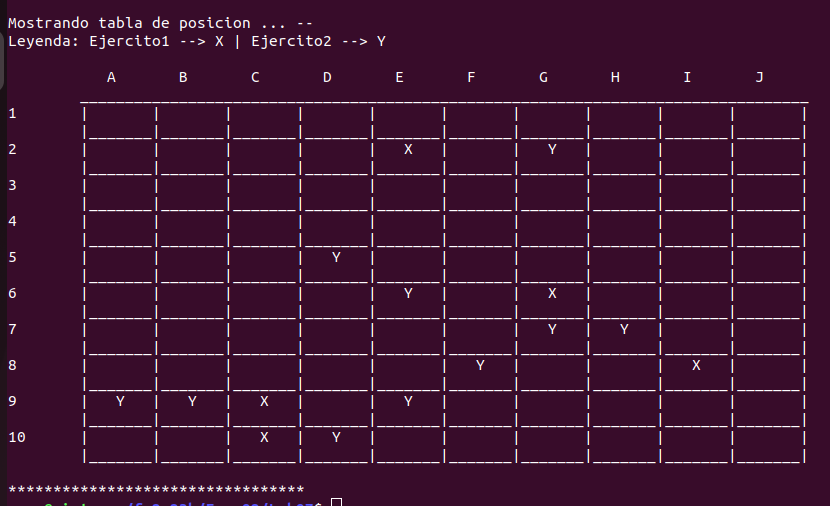
\includegraphics[width=1.0\textwidth,keepaspectratio]{img/Commit4.png}
		%\includesvg{img/automata.svg}
		%\label{img:mot2}
		%\caption{Product backlog.}
	\end{figure}
	\subsection{Estructura de laboratorio 07}
	\begin{itemize}	
		\item El contenido que se entrega en este laboratorio07 es el siguiente:
	\end{itemize}
	\begin{lstlisting}[style=ascii-tree]
	/Lab07	
		"PONER RAMA"
	\end{lstlisting}    
	\section{\textcolor{red}{Rúbricas}}
	
	\subsection{\textcolor{red}{Entregable Informe}}
	\begin{table}[H]
		\caption{Tipo de Informe}
		\setlength{\tabcolsep}{0.5em} % for the horizontal padding
		{\renewcommand{\arraystretch}{1.5}% for the vertical padding
		\begin{tabular}{|p{3cm}|p{12cm}|}
			\hline
			\multicolumn{2}{|c|}{\textbf{\textcolor{red}{Informe}}}  \\
			\hline 
			\textbf{\textcolor{red}{Latex}} & \textcolor{blue}{El informe está en formato PDF desde Latex,  con un formato limpio (buena presentación) y facil de leer.}   \\ 
			\hline 
			
			
		\end{tabular}
	}
	\end{table}
	
	\clearpage
	
	\subsection{\textcolor{red}{Rúbrica para el contenido del Informe y demostración}}
	\begin{itemize}			
		\item El alumno debe marcar o dejar en blanco en celdas de la columna \textbf{Checklist} si cumplio con el ítem correspondiente.
		\item Si un alumno supera la fecha de entrega,  su calificación será sobre la nota mínima aprobada, siempre y cuando cumpla con todos lo items.
		\item El alumno debe autocalificarse en la columna \textbf{Estudiante} de acuerdo a la siguiente tabla:
	
		\begin{table}[ht]
			\caption{Niveles de desempeño}
			\begin{center}
			\begin{tabular}{ccccc}
    			\hline
    			 & \multicolumn{4}{c}{Nivel}\\
    			\cline{1-5}
    			\textbf{Puntos} & Insatisfactorio 25\%& En Proceso 50\% & Satisfactorio 75\% & Sobresaliente 100\%\\
    			\textbf{2.0}&0.5&1.0&1.5&2.0\\
    			\textbf{4.0}&1.0&2.0&3.0&4.0\\
    		\hline
			\end{tabular}
		\end{center}
	\end{table}	
	
	\end{itemize}
	
	\begin{table}[H]
		\caption{Rúbrica para contenido del Informe y demostración}
		\setlength{\tabcolsep}{0.5em} % for the horizontal padding
		{\renewcommand{\arraystretch}{1.5}% for the vertical padding
		%\begin{center}
		\begin{tabular}{|p{2.7cm}|p{7cm}|x{1.3cm}|p{1.2cm}|p{1.5cm}|p{1.1cm}|}
			\hline
    		\multicolumn{2}{|c|}{Contenido y demostración} & Puntos & Checklist & Estudiante & Profesor\\
			\hline
			\textbf{1. GitHub} & Hay enlace URL activo del directorio para el  laboratorio hacia su repositorio GitHub con código fuente terminado y fácil de revisar. &2 &X &2 & \\ 
			\hline
			\textbf{2. Commits} &  Hay capturas de pantalla de los commits más importantes con sus explicaciones detalladas. (El profesor puede preguntar para refrendar calificación). &4 &X &4 & \\ 
			\hline 
			\textbf{3. Código fuente} &  Hay porciones de código fuente importantes con numeración y explicaciones detalladas de sus funciones. &2 &X &2 & \\ 
			\hline 
			\textbf{4. Ejecución} & Se incluyen ejecuciones/pruebas del código fuente  explicadas gradualmente. &2 &X &2 & \\ 
			\hline			
			\textbf{5. Pregunta} & Se responde con completitud a la pregunta formulada en la tarea.  (El profesor puede preguntar para refrendar calificación).  &2 &X &2 & \\ 
			\hline	
			\textbf{6. Fechas} & Las fechas de modificación del código fuente estan dentro de los plazos de fecha de entrega establecidos. &2 &X &2 & \\ 
			\hline 
			\textbf{7. Ortografía} & El documento no muestra errores ortográficos. &2 &X &2 & \\ 
			\hline 
			\textbf{8. Madurez} & El Informe muestra de manera general una evolución de la madurez del código fuente,  explicaciones puntuales pero precisas y un acabado impecable.   (El profesor puede preguntar para refrendar calificación).  &4 &X &2 & \\ 
			\hline
			\multicolumn{2}{|c|}{\textbf{Total}} &20 & &18 & \\ 
			\hline
		\end{tabular}
		%\end{center}
		%\label{tab:multicol}
		}
	\end{table}
	
\clearpage

\section{Referencias}
\begin{itemize}			
	\item \url{https://drive.google.com/file/d/128O7v3wmrnl9g0a6BhMTNMnGIL3jTUDz/view}
\end{itemize}	
	
%\clearpage
%\bibliographystyle{apalike}
%\bibliographystyle{IEEEtranN}
%\bibliography{bibliography}
			
\end{document}